\chapter{Evaluation of the Cloud Scheme}

\section{Introduction}

In this chapter, the simulated climatology from the simple cloud scheme described in \chapref{chp:simple_cld_scheme} is presented here. \secref{sec:exp_setup_and_dataset} introduces the experiment setup and data sets used in this chapter. The evaluation will focus on features of cloud fraction, cloud water path and cloud radiative effects, including their vertical profile (if any), spatial pattern, zonal mean structure and seasonal cycles.

\section{Data and methods}
\label{sec:exp_setup_and_dataset}

\subsection{Experiment setup}

Our simulations are AMIP-type, that is they follow those used in the Atmospheric Model Intercomparison Project. They are performed with a realistic Earth-continental configuration following \citet{Thomson2018} (which is derived from the ERA-Interim land mask and topography \citep{Dee2011}) and at a horizontal resolution of T42 (roughly 2.8$^\circ$ $\times$ 2.8$^\circ$) with 25 vertical levels. The sea surface temperature is fixed at AMIP climatology \citep{Taylor2000sea}, which is annually repeating but seasonally varying. The sea ice data is also from AMIP, but is averaged over all years and months to obtain an annual mean distribution, as in \citet{Thomson2018}. The albedo in sea ice regions increases linearly with the sea ice concentration with the maximum of 0.7. The surface albedo of the other parts except the sea ice is fixed as 0.11. The insolation includes a seasonal and diurnal cycle, with a solar constant of 1360 Wm$^{-2}$. The convection parameterization used in this study is the simplified Betts--Miller scheme from \citet{Frierson2007}. 

The SOCRATES (Suite of Community Radiation Codes based on Edwards \& Slingo) radiation scheme \citep{Edwards1996, Manners2015} is employed for the radiation transfer calculation as in \citet{Thomson2019}. Spectral files with 9 longwave bands and 6 shortwave bands are used, which are those used in the Unified Model's Global Atmosphere version 7 \citep{Walters2019}. The cloud fraction, effective radius of cloud particle and liquid water mixing ratio in each grid are passed to it, then the radiation fluxes under all-sky and clear-sky conditions are obtained, which are used to analyze the energy balance and to calculate the cloud radiative effect \citep{Ramanathan1989, Li2017} at the TOA.

In order to compare the roles of different cloud parameterization schemes, simulations are performed with the combination of different clouds or different adjustment methods as shown in Table \ref{tab:exps}. The simulation with large-scale clouds only is denoted as the LS simulation. The run with large-scale clouds and freeze-dry adjustment is called the FD simulation. The run performed with large-scale clouds, freeze-dry adjustment and marine low stratiform clouds is referred as the ALL simulation. The simulations are all run for 20 years, with the first 10 years treated as spin-up and discarded.

\begin{table}
	\caption{Summary of the Isca fixed-SST simulations}
	\vspace{0.5em}
	\centering
	\renewcommand{\arraystretch}{1.3}
	\begin{tabular}{ll}
		\hline
		Experiment & Description \\
		\hline
		LS  & Run with large-scale clouds only. \\ 
		FD  & Based on the LS run, with freeze-dry adjustment also applied. \\ 
		\multirow{2}{*}{ALL} & The marine low-level clouds are also included on top of the \\
		    & FD run.  \\
		\multirow{3}{*}{Linear\_X} 	&  X is one of the LS, FD and ALL runs, in which the large-scale \\
		& clouds are diagnosed from a linear function of RH as defined\\
		& in \eqref{eq:linear_cf_rh}. \\
		\multirow{2}{*}{Sundqvist\_X} & Same as Linear\_X, but with \citet{Sundqvist1989} scheme\\ 
		& as defined in \eqref{eq:sundqvist}.\\
		\hline
	\end{tabular}
	\label{tab:exps}
\end{table}

\subsection{Data sets}
To evaluate the performance of the cloud scheme, several observations and reanalysis data sets are employed. Specifically, the 10-year monthly data (1995 to 2014) of International Satellite Cloud Climatology Project (ISCCP) H-series products \citep{Young2018} is used to evaluate the simulated cloud amounts. The cloud fraction from Isca simulations is compared to retrieved cloud fraction from GCM-Oriented Cloud-Aerosol Lidar and Infrared Pathfinder Satellite Observations (CALIPSO) Cloud Observations product (GOCCP) \citep{Chepfer2010}. To examine the radiative flux simulated in Isca, monthly data from January 2001 to December 2018 from Clouds and Earth's Radiant Energy System (CERES) Energy Balanced and Filled (EBAF) Edition 4.1 product \citep[CERES-EBAF hereafter;][]{Loeb2018} are used for comparison. The cloud water path is from the CloudSat 2B-CWC-RO Release P1\_R05 data product \citep{Austin2009} from 2012 to 2016, which can better represent cloud liquid and ice water path over high latitudes than CERES-EBAF data set, owing to its explicit determination of cloud phase \citep{Lenaerts2017}. In addition, monthly vertical pressure velocity from ERA-Interim reanalysis and radiative flux data from CERES-EBAF data sets covering the period 2008-2017 are also adopted to quantify the longwave CRE over the tropics.

In order to demonstrate how this cloud scheme performs with respect to more comprehensive models, the monthly mean radiative fluxes at clear-sky and all-sky conditions in historical simulation (1996 to 2005) from various CMIP5 models are also shown for the names of models). All the data sets are remapped to T42 resolution when necessary for a direct comparison with Isca simulations.

\section{Simulated cloud amount}
\label{sec:cld_amt}

The global mean cloud amount and radiative components for the observations and Isca simulations are summarized in Table \ref{tab:global_mean_climate}. 

\begin{sidewaystable}
	\caption{Global and annual mean climatological properties of observations and different Isca simulations, which are summarized in Table \ref{tab:exps}. The net fluxes in the table are positive downward. }
	\vspace{0.5em}
	\centering
	\renewcommand{\arraystretch}{1.5}
	% https://tex.stackexchange.com/questions/209802/footnote-in-table-environment
	% use this package for footnote
	\begin{threeparttable}
	%\begin{tabular}{lrrrrrrr}
	\begin{tabular}{lccccccc}
    	\hline
    	{} &   Obs &  Linear\_LS &  Linear\_FD &  Linear\_ALL &  Sundqvist\_LS &  Sundqvist\_FD &  Sundqvist\_ALL \\
    	\hline
    	Low cloud amount (\%)      &  28.0\tnote{a} &       54.6 &       49.3 &        48.6 &          53.8 &          48.3 &           47.5 \\
    	Middle cloud amount (\%)   &  20.8\tnote{a} &       25.9 &       20.8 &        20.6 &          25.3 &          20.2 &           20.0 \\
    	High cloud amount (\%)     &  12.8\tnote{a} &       42.3 &       30.4 &        30.4 &          35.9 &          25.5 &           25.5 \\
    	Total cloud amount (\%)    &  65.3\tnote{a} &       75.6 &       66.4 &        66.0 &          72.4 &          63.3 &           62.6 \\
    	TOA net SW flux (Wm$^{-2}$)  & 241.3\tnote{b} &      226.8 &      229.2 &       229.6 &         228.7 &         231.2 &          231.5 \\
    	TOA net LW flux (Wm$^{-2}$)  & 240.3\tnote{b} &      220.4 &      224.8 &       224.9 &         223.3 &         227.6 &          227.4 \\
    	TOA net flux (Wm$^{-2}$)     &   1.0\tnote{b} &        6.4 &        4.5 &         4.7 &           5.4 &           3.6 &            4.0 \\
    	TOA SW CRE (Wm$^{-2}$)       & -45.8\tnote{b} &      -58.8 &      -56.3 &       -56.0 &         -56.9 &         -54.3 &          -54.1 \\
    	TOA LW CRE (Wm$^{-2}$)       &  28.0\tnote{b} &       36.4 &       31.3 &        31.0 &          33.3 &          28.5 &           28.3 \\
    	TOA net CRE (Wm$^{-2}$)      & -17.8\tnote{b} &      -22.4 &      -25.0 &       -24.9 &         -23.5 &         -25.8 &          -25.8 \\
    	Cloud water path (gm$^{-2}$) & 119.3\tnote{c} &      147.0 &      129.7 &       130.4 &         144.1 &         127.1 &          126.8 \\
    	\hline
    \end{tabular}
    
    \begin{tablenotes}
      \item[a] The observed cloud amounts are from ISCCP H-series \citep{Young2018} product (1995--2014)
      \item[b] The radiative fluxes and cloud radiative effects (CREs) at the TOA are from CERES-EBAF \citep{Loeb2018} data set (2001--2018)
      \item[c] The cloud water path is from CloudSat 2B-CWC-RO Release P1\_R05 \citep{Austin2009} data product (2012--2016)
     \end{tablenotes}
     
    \end{threeparttable}
    \label{tab:global_mean_climate}
\end{sidewaystable}

The global mean cloud fraction profiles from CALIPSO-GOCCP, ERA-Interim reanalysis and Isca simulations are displayed in \figref{fig:cld_fraction_profile}a. The cloud fractions from all the Isca simulations are higher than observations, especially in the middle and high levels. The FD simulations are closer to observations than the LS simulations, which is true for both the linear and Sundqvist schemes. Regarding the annual and zonal mean profiles, a striking feature is that the LS simulations from both linear and Sundqvist schemes overestimate the cloud fraction at high latitudes (\figsref{fig:cld_fraction_profile}d and \ref{fig:cld_fraction_profile}g) compared to the observation (\figref{fig:cld_fraction_profile}b) and reanalysis (\figref{fig:cld_fraction_profile}c). These biases are mitigated in the FD simulations (\figsref{fig:cld_fraction_profile}e and \ref{fig:cld_fraction_profile}h), as the cloud fractions are limited due to insufficient water vapor content at high latitudes. Despite more clouds being diagnosed at low levels over the eastern subtropical ocean regions, the zonal mean cloud fraction profiles in the ALL simulations (\figsref{fig:cld_fraction_profile}f and \ref{fig:cld_fraction_profile}i) are generally similar to those from the FD simulations. In summary, the cloud fraction profiles have been improved from the LS to ALL simulations due to the freeze-dry adjustment and the extra low clouds. However, the cloud fractions are still overestimated in high levels over the subtropics, which could possibly explain the CRE biases over these regions.

\begin{figure}[ht]
	\centering
	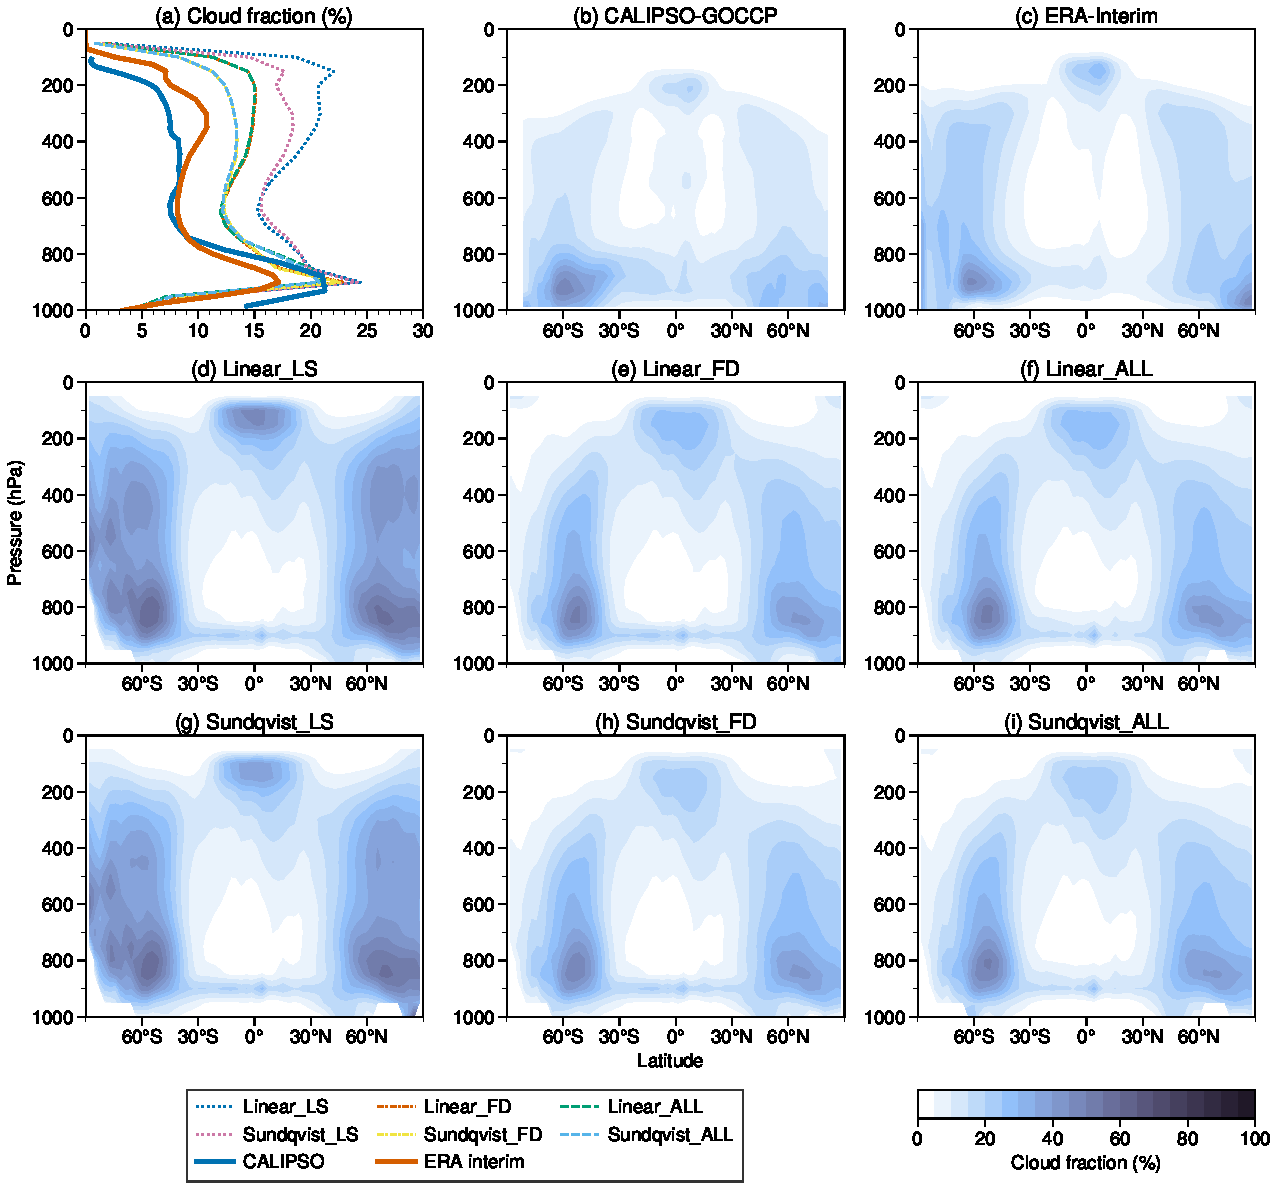
\includegraphics[width=1.\linewidth]{{figs/evaluation_of_cld_scheme/cloud_zonal_mean_vert_profiles}.pdf}
	\caption{(a) The annual and global mean of cloud fraction profiles from the CALIPSO-GOCCP (thick blue solid line), ERA-Interim reanalysis (thick orange solid line) and different Isca simulations, including linear\_LS (blue dotted), linear\_FD (orange dash-dotted), linear\_ALL (green dashed), Sundqvist\_LS (pink dotted), Sundqvist\_FD (yellow dash-dotted) and Sundqvist\_ALL (azure dashed). (b-i) Same as in (a), but for annual and zonal mean of cloud fraction profiles.}
	\label{fig:cld_fraction_profile}
\end{figure}

In addition to the cloud fraction profiles, the geographic patterns of cloud amount, diagnosed from the random-maximum overlap assumption (\secref{sec:cld_amt_diag}), are also compared with observations. For example, the annual mean spatial patterns of low cloud amount from three different simulations (LS, FD and ALL) with linear RH cloud scheme, ISCCP-H data set, and the differences between them are shown in \figref{fig:low_cld_amt}. It should be pointed out that the simulated cloud amounts are compared to the satellite retrievals directly in this study, because the cloud simulator \citep[e.g.,][]{Bodas2011} has not been implemented in Isca. This may bring in some inconsistencies, but it does provide a useful first look of the cloud amount diagnosis.

\begin{figure}[ht]
	\centering
	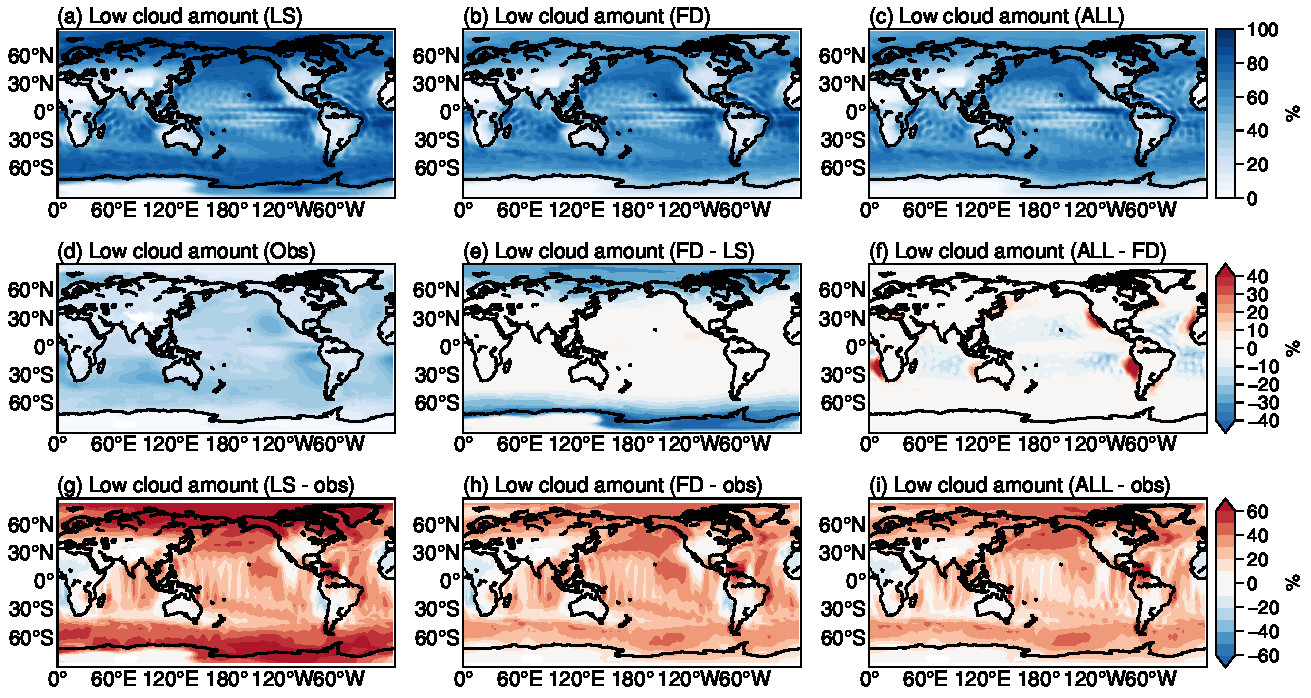
\includegraphics[width=1\linewidth]{{figs/evaluation_of_cld_scheme/low_cld_amt_isca_obs}.pdf}
	\caption{The annual mean geographic patterns of low cloud amount (\%) from the (a) LS, (b) FD, (c) ALL simulations with the linear scheme as well as (d) observation (ISCCP-H), and the differences between the (e) FD and LS, (f) ALL and FD, (g) LS and observation, (h) FD and observation, and (i) ALL and observation. Note that (a-d) use the upper color scale, (e-f) use the middle one, and (g-i) use the one at the bottom.}
	\label{fig:low_cld_amt}
\end{figure}

One evident feature of the low cloud amount in observations is that marine stratocumulus clouds dominate the areas off the west coast of continents (\figref{fig:low_cld_amt}d), related to the subsidence branch of the Hadley Cell \citep{Wood2012}. The predominantly downward motion in these regions generally suppresses cloud formation in the middle and upper troposphere, but due to the abundance of water vapor near the ocean surface, clouds form at the top of convective boundary layers. However, these marine low clouds are too far from the coasts in the LS simulation compared to the observations (\figref{fig:low_cld_amt}a). Looking at the differences between LS simulation and observations (\figref{fig:low_cld_amt}g), the low cloud amount is underestimated by about 20\% off the west coast of Peru. In fact, these are well-known biases in CMIP5 models \citep{Dolinar2015}. Another problem of the LS simulation is the overproduction of low cloud amount in polar regions (\figref{fig:low_cld_amt}g). For example, LS simulation produces more than 40\% low cloud over Arctic region. %which is a similar but less severe bias in mid-latitudes.

In contrast, the cloud fractions in the FD and ALL simulations are adjusted by the freeze-dry method (see \secref{sec:freezedry}), which is mainly designed to reduce the unrealistic cloud amount in polar regions. Thus there is a reduction of low cloud amount over high latitudes in these two simulations (\figsref{fig:low_cld_amt}h and \ref{fig:low_cld_amt}i), although some positive biases still exist there. Compared with the LS simulation directly, the FD simulation can reduce the low cloud amount by more than 20\% over polar regions (\figref{fig:low_cld_amt}e), showing a better agreement with the observations. The ALL simulation can further diagnose the marine stratus clouds off the west coast of continents through the predictor ELF, making the low clouds distribution closer to the observation (\figref{fig:low_cld_amt}c). It is noted that pronounced changes occur off the west coasts of Peru, California and Namibia in the ALL simulation, where the cloud fraction increases over 20\% (\figref{fig:low_cld_amt}f) than the FD run. As shown in Table \ref{tab:global_mean_climate}, the global mean low cloud amount decreases from 54.6\% to 48.6\% from the LS to ALL simulations with the linear RH scheme, which is closer to the observed value (28\%). The changes of total cloud amount in these simulations (not shown here) are similar, and the global mean value decreases from 75.6\% (the LS run) to 66.0\% (the ALL run) for the linear RH scheme (Table \ref{tab:global_mean_climate}).

\begin{figure}[ht]
	\centering
	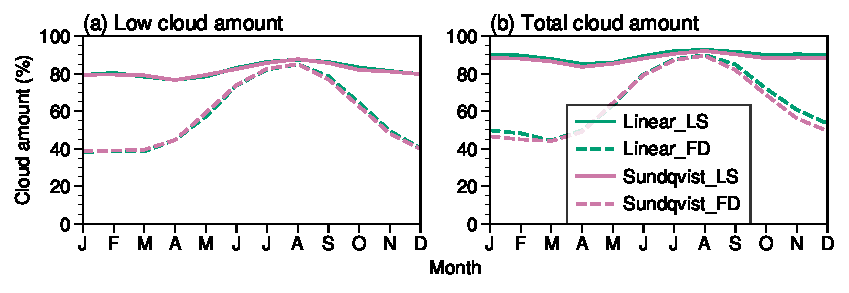
\includegraphics[width=1.0\linewidth]{{figs/evaluation_of_cld_scheme/cloud_amount_in_arctic_region}.pdf}
	\caption{The seasonal cycle of (a) low and (b) total cloud amount (\%) over the Arctic region ($60^\circ$-$90^\circ$N) from the LS (solid lines) and FD (dashed lines) simulations, where the freeze-dry adjustment method is applied in the FD simulations. The green and pink colors denote the experiments performed with the linear and Sundqvist cloud schemes respectively.}
	\label{fig:cld_amt_freeze-dry}
\end{figure}

The above analyses have shown that the freeze-dry method can improve the spatial patterns of annual mean cloud amount, with these changes being especially pronounced  during winter time \citep[as also noted by][]{Vavrus2008}. Figure \ref{fig:cld_amt_freeze-dry} illustrates the annual cycle of low and total cloud amounts over Arctic region from both linear RH and Sundqvist schemes. In the LS simulations, both the low and total cloud amounts are nearly at the same level throughout the year. However, a striking feature in the FD simulations is that the cloudiness declines rapidly during boreal winter but remains almost unchanged in warm and moist summer, which in fact is more realistic compared to observations as pointed by \citet{Vavrus2008}.


\section{Simulated cloud water path}
\label{sec:cwp}

\begin{figure}[ht]
	\centering
	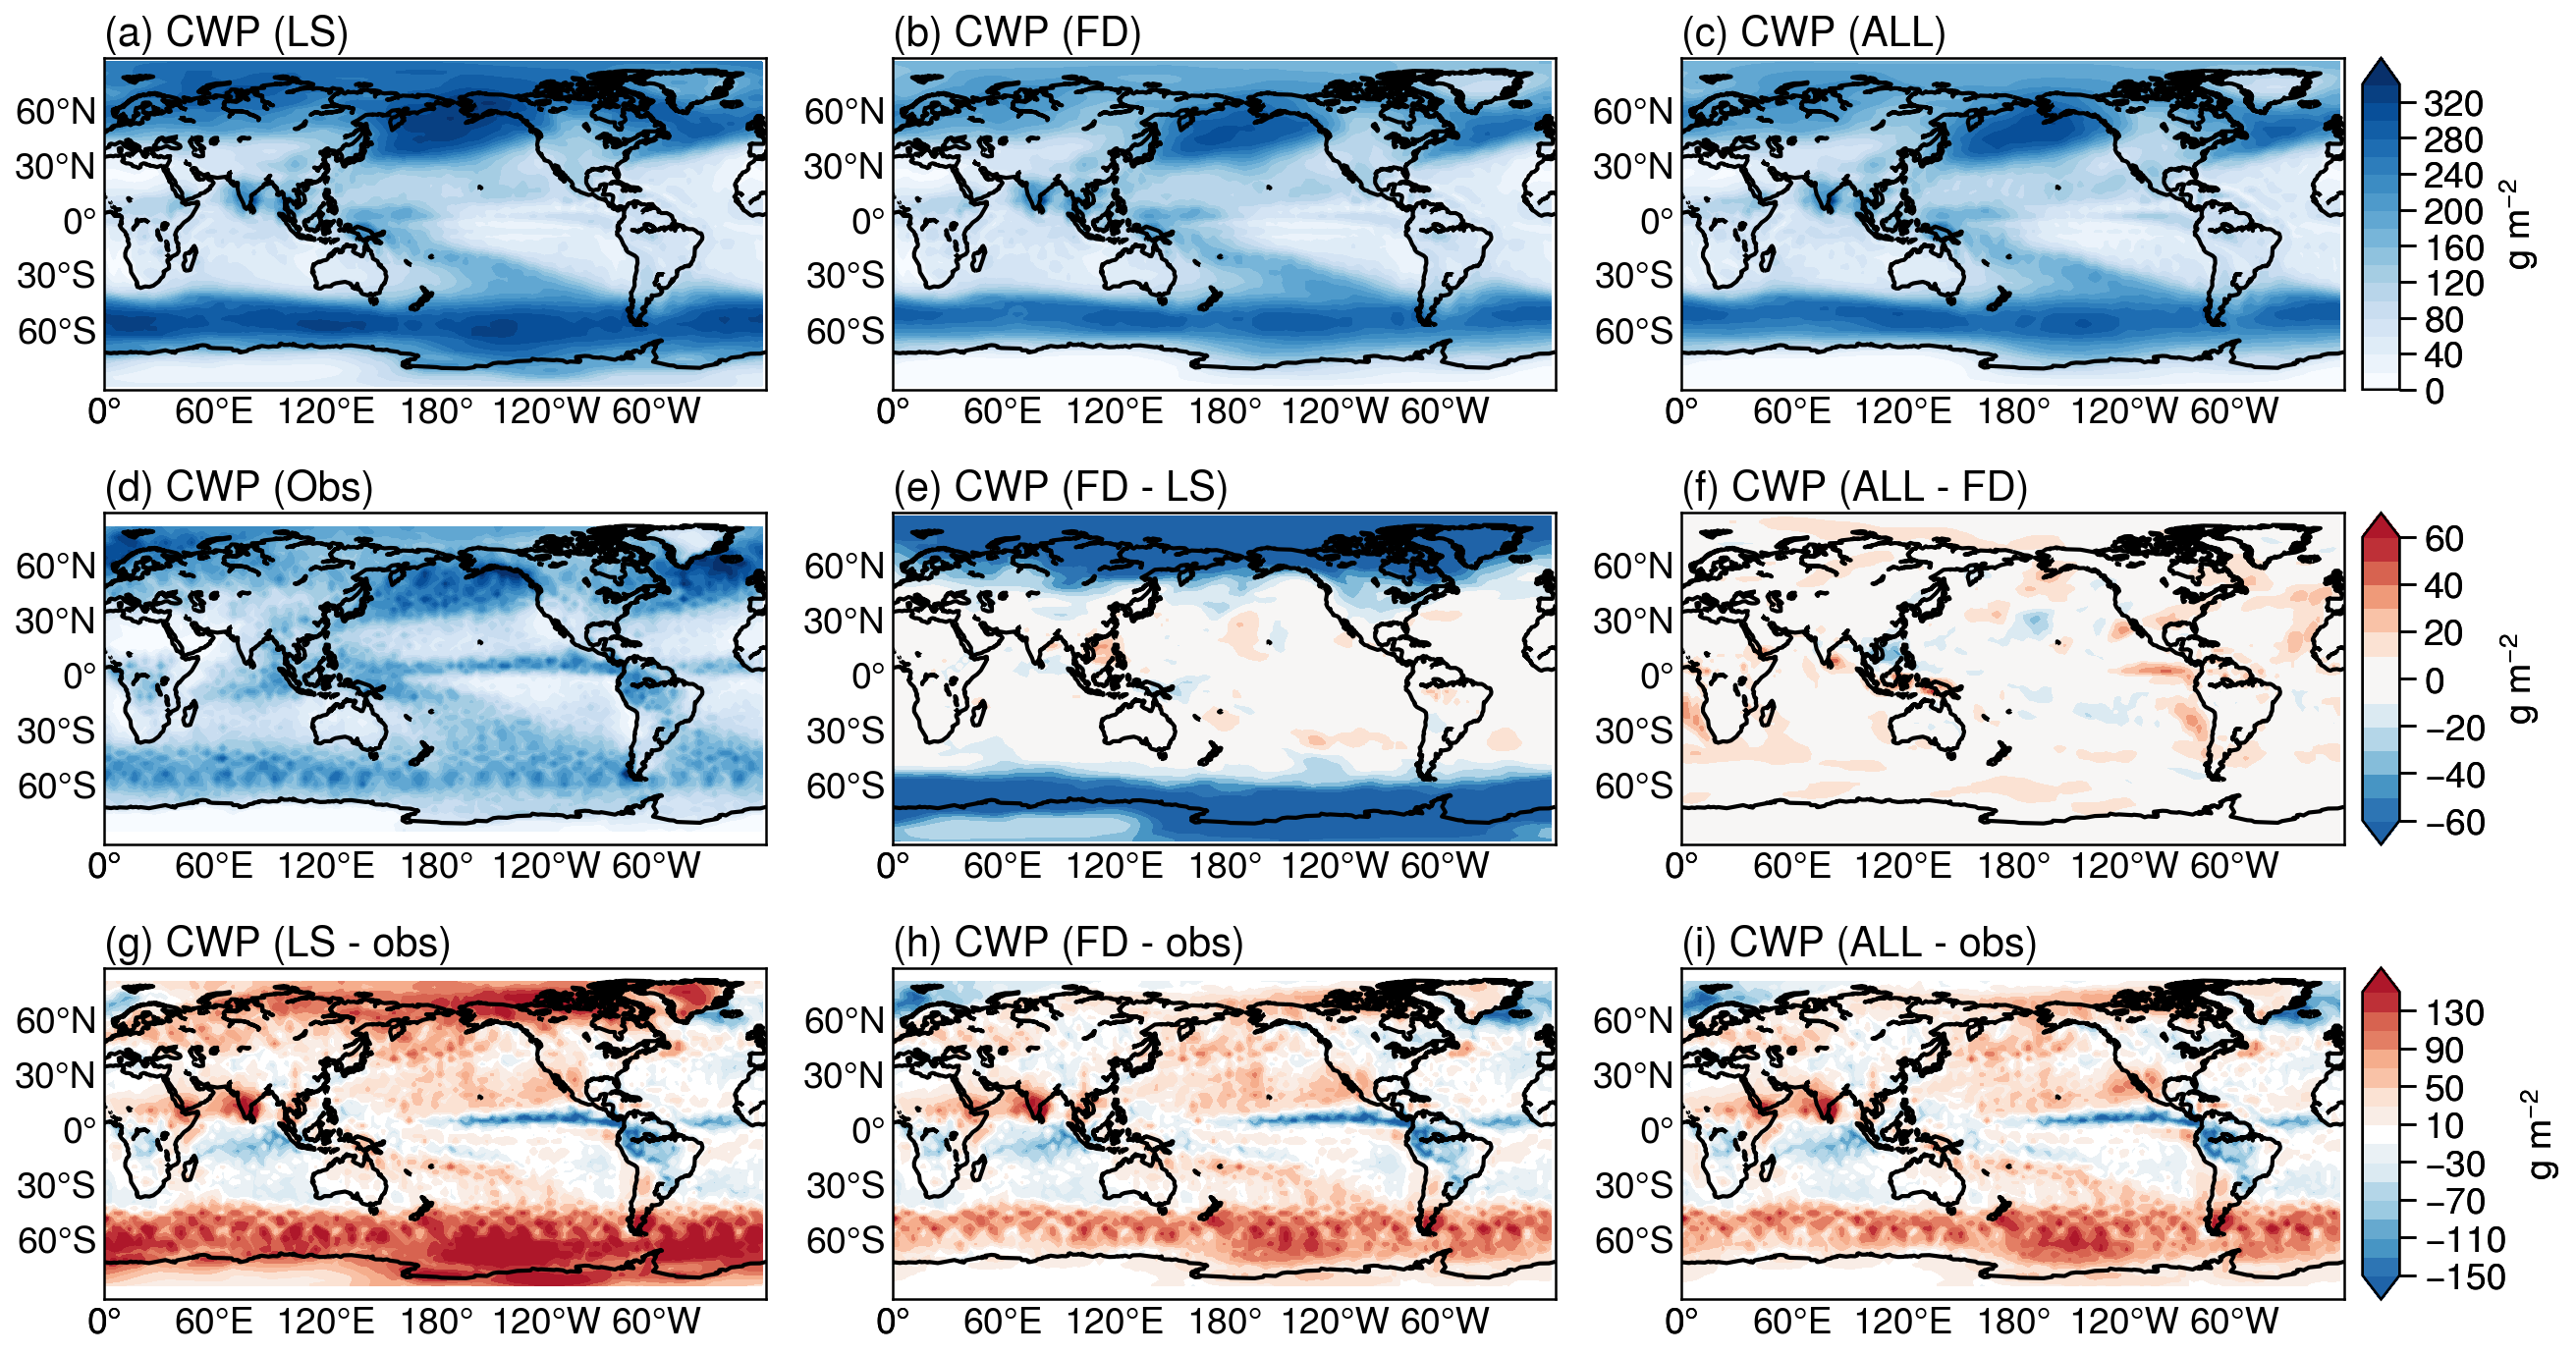
\includegraphics[width=1\linewidth]{{figs/evaluation_of_cld_scheme/cwp_isca_obs}.pdf}
	\caption{Same as \figref{fig:low_cld_amt}, but for the spatial patterns of total cloud water path (CWP; gm$^{-2}$). The observed climatology of CWP is derived from the CloudSat data set.}
	\label{fig:cwp}
\end{figure}

The cloud water path (CWP) measures the total amount of cloud water within a column and is defined as the integral of cloud water content from surface ($p=p_s$) to TOA ($p=0$) \citep[Eq. 9.30 in][]{Stensrud2009}, and it can be expressed as follows if the hydrostatic equilibrium is assumed:
\begin{equation}
	CWP = \int_{p=0}^{p=p_s} C\cdot q_l\frac{dp}{g},
	\label{eq:cwp}
\end{equation}
where $q_l$ is the in-cloud liquid water mixing ratio specified in Equation (\ref{eq:qcl}), $C$ is the cloud fraction within a grid box, $g$ is the acceleration due to gravity and $p$ is the pressure. The global and annual mean CWP in the LS simulation from linear RH scheme is 147.0 gm$^{-2}$, which is larger than the observed global mean result (119.3 gm$^{-2}$, see Table \ref{tab:global_mean_climate}). As displayed in \figref{fig:cwp}, one obvious bias in the spatial pattern in the LS simulation is the overestimation of CWP at high latitudes. For instance, these biases can be even more than 90 gm$^{-2}$ in the polar regions (\figsref{fig:cwp}a and \ref{fig:cwp}g). Such an overestimation is also evident in cloud amount over the polar regions (e.g. \figref{fig:low_cld_amt}g), suggesting that the adjustment of cloud fraction probably reduces the CWP biases there. Indeed, incorporating the freeze-dry method into the simulation produces a large change in the CWP spatial pattern, with a reduction over 60 gm$^{-2}$ over polar regions (\figsref{fig:cwp}b, \ref{fig:cwp}e and \ref{fig:cwp}h). The CWP biases off the west coast of continents are reduced in the ALL simulation due to the increase of the low cloud fraction there. For example, the CWP over Peruvian and Californian coasts in the ALL simulation increases at least 20 gm$^{-2}$ when compared to the LS simulation (\figref{fig:cwp}e).

\section{Simulated cloud radiative effect}

\begin{figure}[ht]
	\centering
	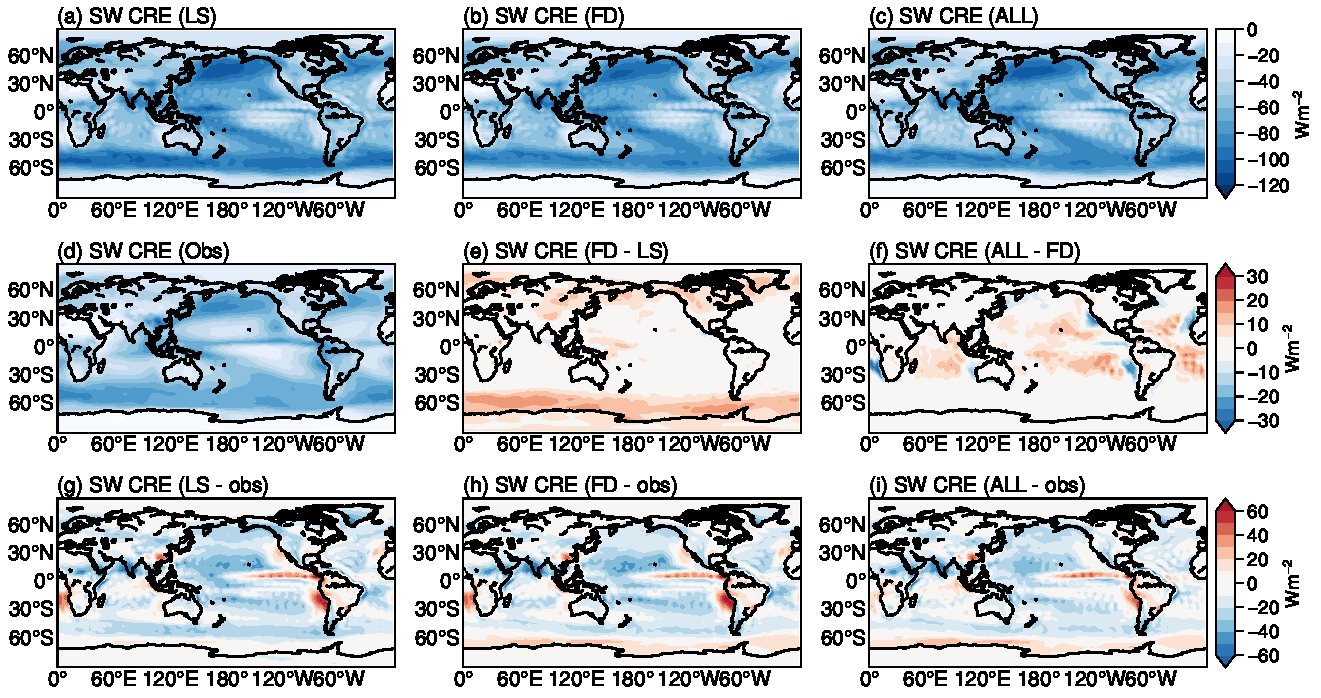
\includegraphics[width=1\linewidth]{{figs/evaluation_of_cld_scheme/toa_sw_cre_isca_obs}.pdf}
	\caption{Same as \figref{fig:low_cld_amt}, but for shortwave (SW) cloud radiative effect (CRE) (Wm$^{-2}$) at TOA. The observed SW CRE is from CERES-EBAF data set.}
	\label{fig:toa_sw_cre}
\end{figure}

\begin{figure}[ht]
	\centering
	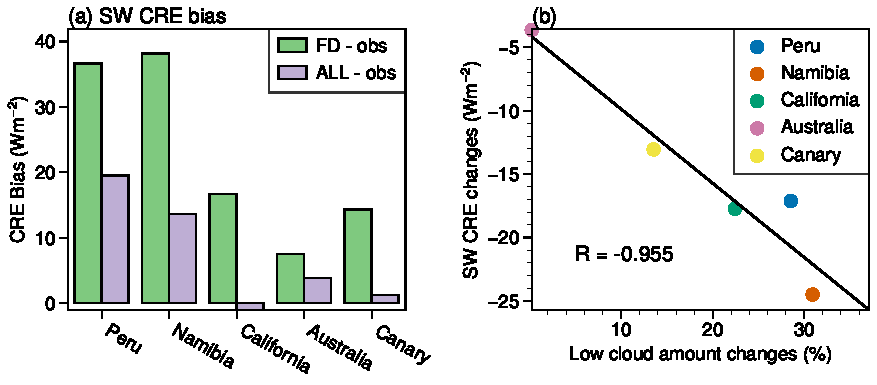
\includegraphics[width=1.\linewidth]{{figs/evaluation_of_cld_scheme/SW_CREs_improvement_linear}.pdf}
	\caption{(a) The regional mean SW CRE biases from the FD and ALL simulations with with linear RH scheme in five different subtropical ocean regions off the west coast of continents, whose ranges are defined in the caption of \figref{fig:fit_low_cld_proxy}. (b) The relationship of regional mean SW CRE and low cloud amount changes in the FD and ALL simulations, and the changes are calculated as their differences (i.e., ALL-FD).}
	\label{fig:swcre_marine_sc}
\end{figure}

The CRE is defined as the differences in TOA radiative fluxes between clear-sky and all-sky conditions \citep[e.g.,]{Ramanathan1989,Li2017}. Specifically, the simulated LW CRE is derived from the difference between the outgoing longwave radiation flux under clear-sky and all-sky conditions, and the SW CRE is computed from the difference in reflected SW flux under clear-sky and all-sky conditions. The net CRE is defined as the sum of LW and SW CREs.

\subsection{Spatial patterns of cloud radiative effect}

The global mean SW CRE from the LS simulation is -58.8 Wm$^{-2}$, which is much larger than the observed value of -45.8 Wm$^{-2}$ from CERES-EBAF (Table \ref{tab:global_mean_climate}). Compared to the observed SW CRE (\figref{fig:toa_sw_cre}c), the LS simulation can reproduce the general features of spatial patterns (\figref{fig:toa_sw_cre}a), although it fails to grasp some key features. For example, SW CRE is underestimated by over 30 Wm$^{-2}$ in eastern subtropical ocean basins off the west coast of Peru and over 15 Wm$^{-2}$ off the west coast of California (\figref{fig:toa_sw_cre}g), consistent with the insufficient low cloud amounts in these marine stratocumulus areas (\figref{fig:low_cld_amt}g). These biases also exist in the FD simulation (\figsref{fig:toa_sw_cre}b and \ref{fig:toa_sw_cre}h), as the freeze-dry method can only adjust the cloud amount over high latitudes. As shown in sections \ref{sec:cld_amt} and \ref{sec:cwp}, the low cloud amount and CWP in these regions increase in the ALL simulation, which is thus expected to improve the SW CRE biases. In fact, the differences between the ALL and FD simulations show that the SW CREs reduce by more than 10 Wm$^{-2}$ off the Californian, Peruvian and Namibian coasts (\figref{fig:toa_sw_cre}f). Consequently, the positive biases in SW CRE over eastern subtropical ocean regions are reduced, although some smaller positive biases still remain (\figref{fig:toa_sw_cre}i). The SW CRE biases from the LD and ALL simulations in the five marine stratocumulus clouds regions (defined in \figref{fig:fit_low_cld_proxy}) are quantified in \figref{fig:swcre_marine_sc}a. It is clear that these biases are reduced in all the locations, which is closely linked to the increase of low cloud amount over these regions (\figref{fig:swcre_marine_sc}b).

Another problem of the SW CRE in the LS simulation is that it is too negative in trade wind cumulus regions, Southern Ocean and northern Pacific Ocean (\figref{fig:toa_sw_cre}g), which is associated with the excessive clouds over these regions (\figref{fig:low_cld_amt}g). The freeze-dry adjustment has reduced the cloud amount at high latitudes, making the SW CRE in the Southern Ocean less negative compared to the LS simulation (\figsref{fig:toa_sw_cre}e and \ref{fig:toa_sw_cre}h). In the end, the SW CRE in the ALL simulation becomes more realistic compared to observations, and the global mean value (-56.0 Wm$^{-2}$) is closer to the observed value (-45.8 Wm$^{-2}$) from CERES-EBAF (Table \ref{tab:global_mean_climate}).

\begin{figure}[ht]
	\centering
	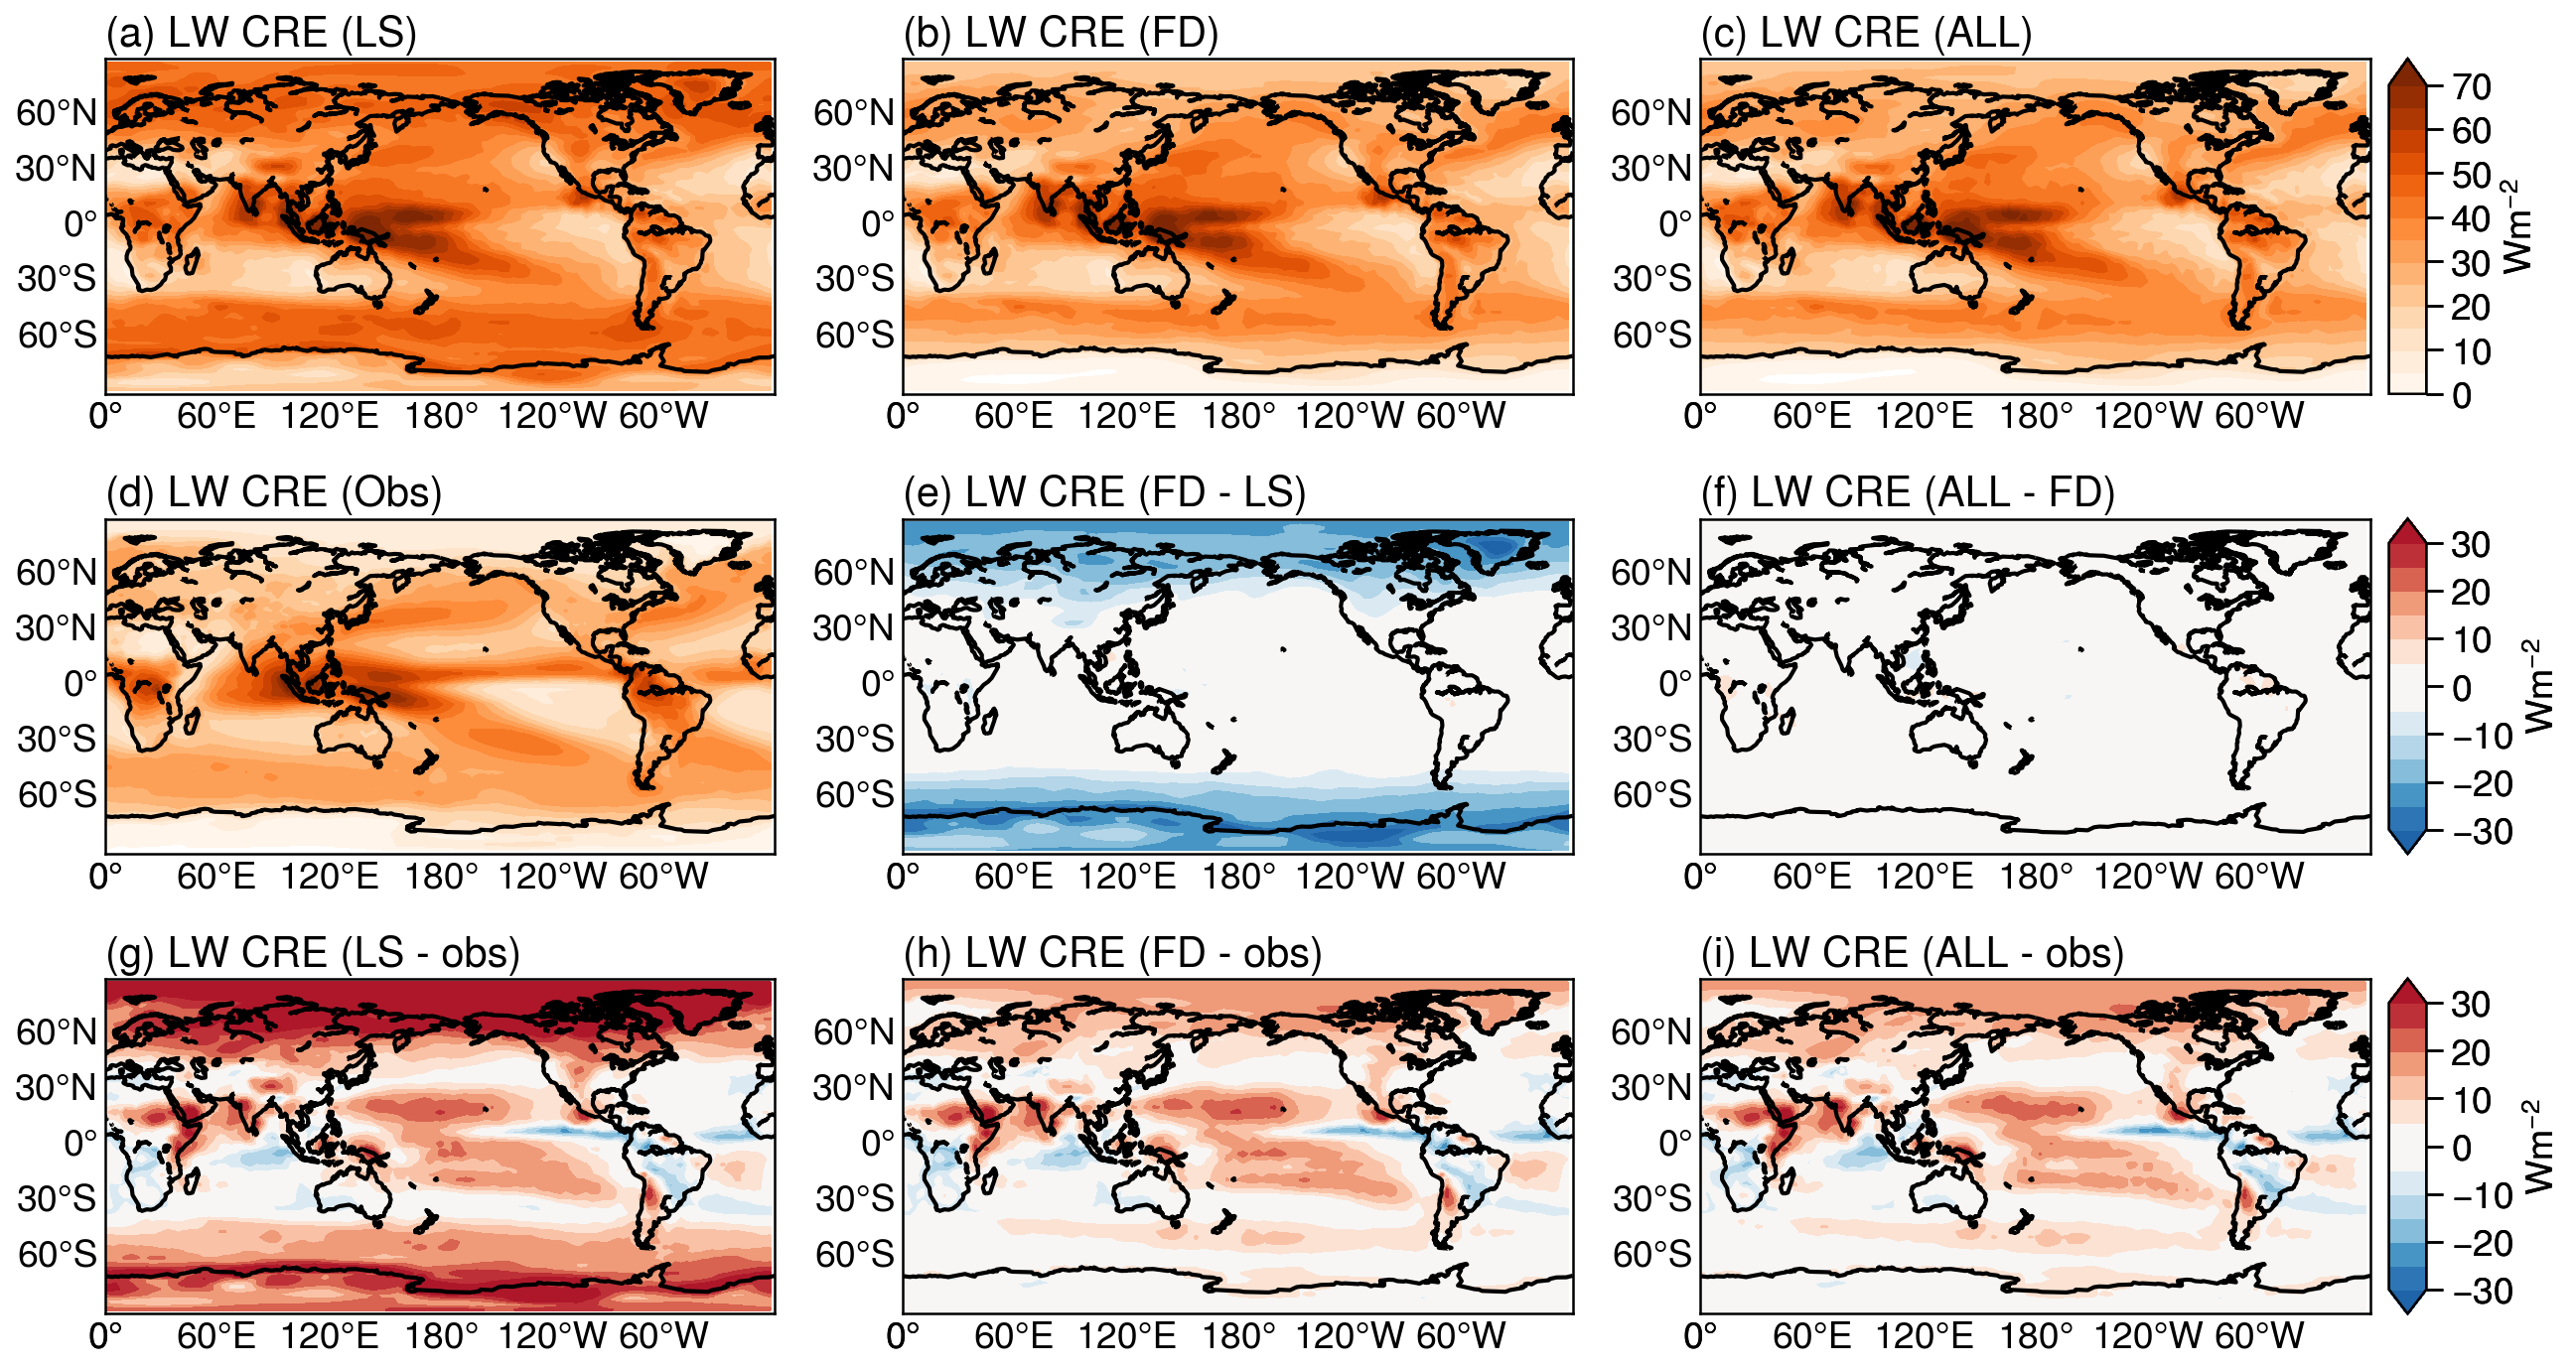
\includegraphics[width=1.\linewidth]{{figs/evaluation_of_cld_scheme/toa_lw_cre_isca_obs}.pdf}
	\caption{Same as \figref{fig:toa_sw_cre}, but for LW CRE (Wm$^{-2}$) at TOA. }
	\label{fig:toa_lw_cre}
\end{figure}

The LS simulation reproduces the general spatial pattern of the observed LW CRE (\figsref{fig:toa_lw_cre}a and \ref{fig:toa_lw_cre}d). However, the radiative effect is too strong, especially in the polar regions and also over the maritime continent regions (\figsref{fig:toa_lw_cre}a and \ref{fig:toa_lw_cre}d), which is also illustrated by the positive biases over these regions (\figref{fig:toa_lw_cre}g). The LW CRE in the LS simulation is overestimated by over 30 Wm$^{-2}$ in the Arctic and over 15 Wm$^{-2}$ in tropical regions. As discussed in previous sections, the cloud fraction, as well as the CWP in polar regions, decreases in the FD simulation compared to the LS run. Therefore, the LW CRE is improved over these regions (\figsref{fig:toa_lw_cre}b and \ref{fig:toa_lw_cre}h), where the bias in polar region is reduced by more than 15 Wm$^{-2}$ (\figref{fig:toa_lw_cre}e). Nevertheless, there is still a small positive bias over the Arctic and tropical regions. Compared to the FD simulation, the changes in the ALL simulation has little effect on LW CRE (\figref{fig:toa_lw_cre}f). After these improvements, the spatial patterns of LW CRE in the FD and ALL simulations become more similar to the observations, and the global mean CRE drops from 36.4 Wm$^{-2}$ to 31.0 Wm$^{-2}$, much closer to global mean result from observations (Table \ref{tab:global_mean_climate}).

\begin{figure}[ht]
	\centering
	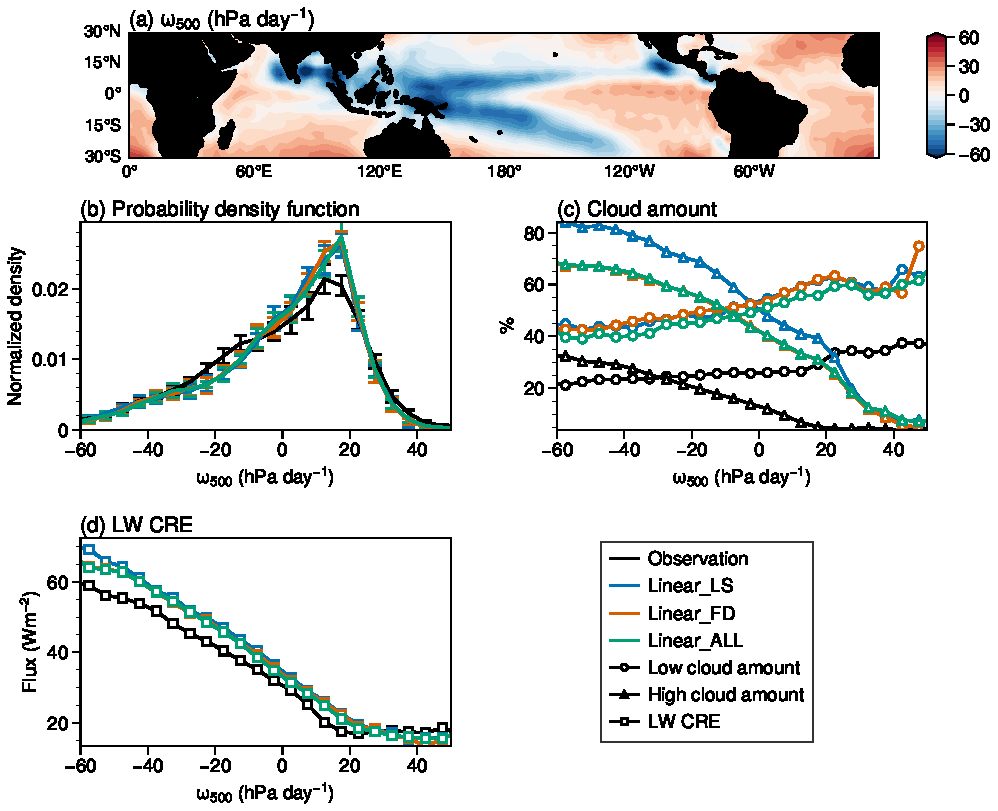
\includegraphics[width=1\linewidth]{{figs/evaluation_of_cld_scheme/linear_cldamt_lwcre_binned_by_omega_year_ocean}.pdf}
	\caption{(a) The vertical pressure velocity field at 500 hPa ($\omega_{500}$) over tropical oceans between 30$^\circ$S and 30$^\circ$N from the linear\_LS simulation. (b) The probability density functions (PDFs) of the 500 hPa large-scale vertical velocity ($\omega_{500}$) over the tropical ocean regions defined in (a), where the vertical bars indicate one standard deviation of the annual mean data. (c) The low, high cloud amounts and (d) the TOA LW CRE in different dynamical regimes binned by $\omega_{500}$. The 10-year (2005-2014) observed cloud amounts from ISCCP-H and the LW CRE from CERES-EBAF are binned by $\omega_{500}$ from ERA-Interim reanalysis data set (black lines). The results from the LS, FD and ALL simulations with the linear RH scheme are represented by blue, orange and green lines, respectively.}
	\label{fig:pdf_lw_cre}
\end{figure}

To further quantify the simulated LW CRE at TOA over the tropical ocean regions (30$^{\circ}$S-30$^{\circ}$N), following the method employed in \citet{Bony2004} and \citet{Bony2005}, we first define the upwelling and downwelling regimes based on the vertical pressure velocity at 500 hPa ($\omega_{500}$, \figref{fig:pdf_lw_cre}a), and then evaluate the LW CRE over these regimes. $\omega_{500}$ is a measure of the large-scale atmospheric circulation, where the regions with positive $\omega_{500}$ are associated with the subsidence movement, while those with negative $\omega_{500}$ are related to large-scale atmospheric ascent. The PDFs of $\omega_{500}$ from the ERA-Interim reanalysis and Isca simulations (LS, FD and ALL runs) are displayed in \figref{fig:pdf_lw_cre}b. The PDFs of the Isca simulations generally follows the observations, albeit the Isca simulations have more weakly ascending regions and fewer weakly descending regions. The peak values of PDFs are located at 5-20 hPa/day, consistent with the results from \citet{Bony2004}.

Figures \ref{fig:pdf_lw_cre}c and \ref{fig:pdf_lw_cre}d illustrate the high/low cloud amounts and LW CRE at the TOA over different dynamical regimes over tropical oceans, respectively. The observed cloud amount and LW CRE are from ISCCP-H and CERES-EBAF data sets respectively, both covering the period from 2005 to 2014 with the regimes being defined by the $\omega_{500}$ from ERA-Interim. The regimes with stronger convective activity, related to the magnitude of $\omega_{500}$ in ascending regions ($\omega_{500}<0$), usually have a larger amount of high clouds and thus stronger LW CREs. All the LW CREs from the three simulations are close to the observed values over the weak upwelling and subsidence regions. However, the LW CREs from the LS simulation deviate from the observations in strong ascending regions ($\omega_{500}<-20$ hPa day$^{-1}$). Furthermore, this discrepancy increases with the magnitude of $\omega_{500}$ in ascending regions ($\omega_{500}<0$). It is noted that the large biases of LW CRE over ascending regions is reduced slightly in the FD and ALL simulations, associated with the decrease of high clouds over those regimes (\figref{fig:pdf_lw_cre}c). However, the positive biases still exist at the strong convection regions. 

\begin{figure}[ht]
	\centering
	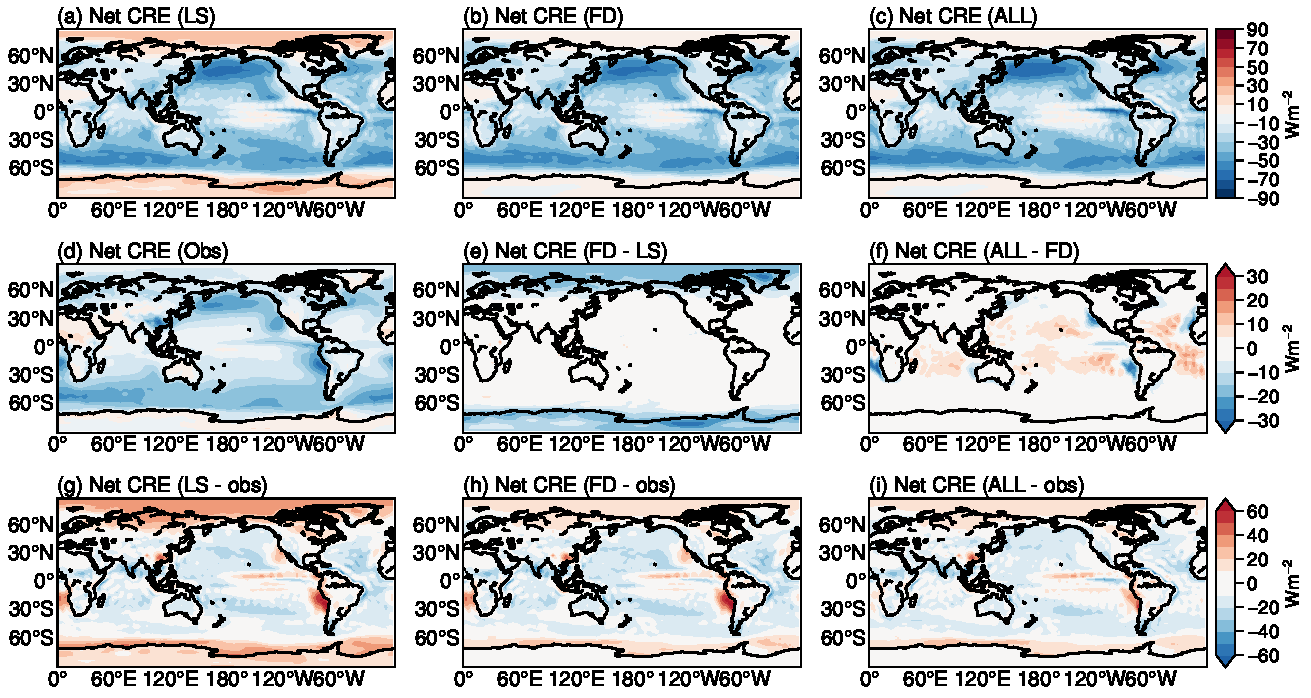
\includegraphics[width=1.\linewidth]{{figs/evaluation_of_cld_scheme/toa_net_cre_isca_obs}.pdf}
	\caption{Same as \figref{fig:toa_sw_cre}, but for net CRE (Wm$^{-2}$) at TOA.}
	\label{fig:toa_net_cre}
\end{figure}

Finally, the spatial pattens of net CREs at the TOA are presented in \figref{fig:toa_net_cre}, where we can see that the positive biases in the LS simulation mainly occur in the polar regions and subtropical eastern ocean regions. There are also small negative biases in subtropical and extratropical regions. The positive biases in net CRE in the LS simulation are related to the cloud amount biases in these regions, as we have seen in the SW and LW CRE fields. Clearly, the biases in polar regions are reduced greatly in the FD simulations (\figsref{fig:toa_net_cre}b, \ref{fig:toa_net_cre}e and \ref{fig:toa_net_cre}h) due to the freeze-dry method. Additionally, the positive biases off the west coasts of continents in subtropics can be mitigated in the ALL simulation (\figref{fig:toa_net_cre}i), making the spatial pattern closer to CERES-EBAF, although there are still slight positive biases in polar regions.

\subsection{Zonal mean structure}
\begin{figure}[ht]
	\centering
	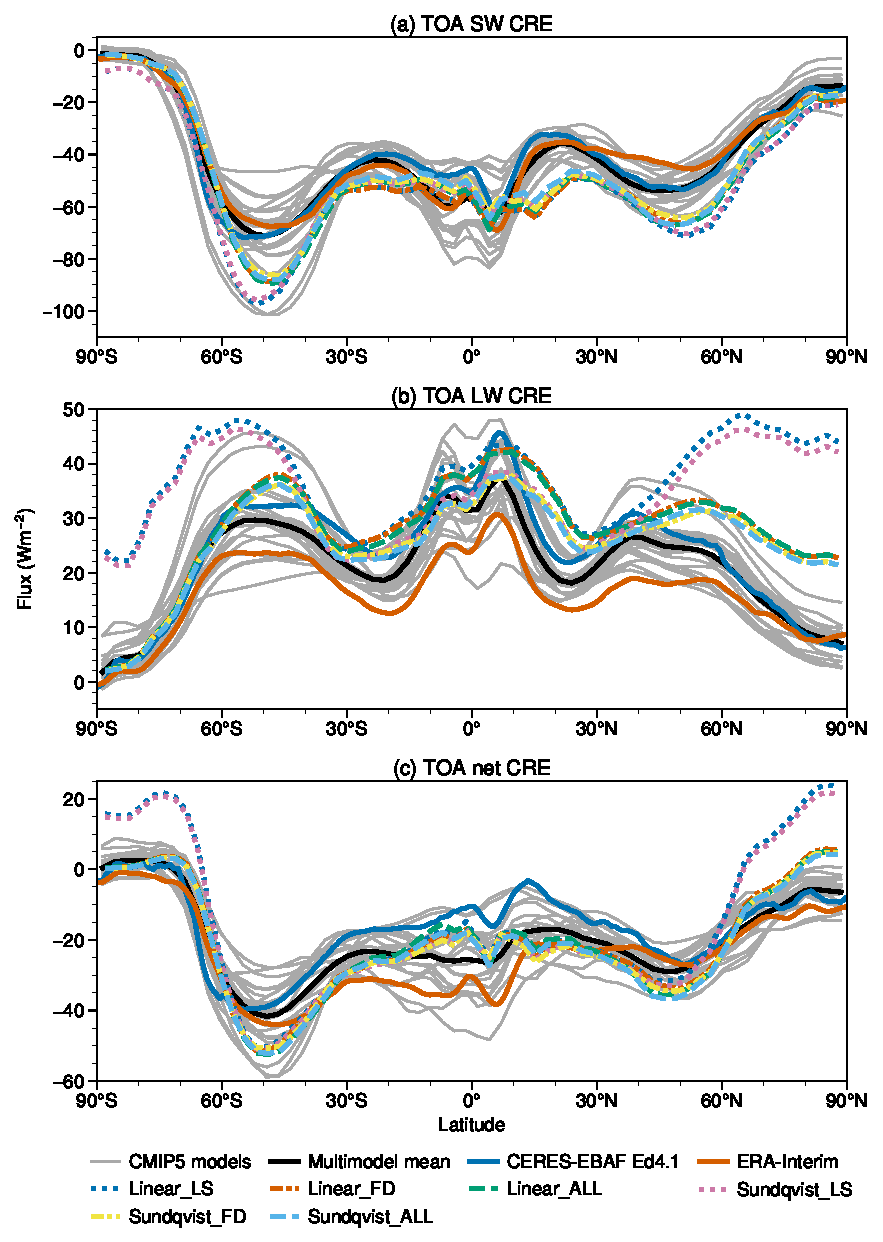
\includegraphics[width=1\linewidth]{{figs/evaluation_of_cld_scheme/cmp_zonal_toa_CRE_cmip_isca}.pdf}
	\caption{Zonally averaged distribution of the TOA (a) SW, (b) LW and (c) net CREs from CERES-EBAF Ed4.1 (blue solid line), ERA-Interim reanalysis (orange solid line), CMIP5 models (thin gray solid lines for each model and black solid line for multimodel mean) and different Isca simulations (dashed/dotted color lines, listed in legend).}
	\label{fig:zonal_mean_cre}
\end{figure}

To further study their latitudinal variations, the zonally averaged SW, LW and net CREs from Isca simulations, CMIP5 simulations, satellite observation and reanalysis data set are shown in \figref{fig:zonal_mean_cre}. For the SW CRE (\figref{fig:zonal_mean_cre}a), the general latitudinal variations can be captured by all the Isca simulations, but the magnitude is larger than observations. The largest discrepancy in the LS simulations occurs in the mid-latitudes, especially in the Southern hemisphere, which is likely arising from the excessive cloud amount over these regions (\figref{fig:low_cld_amt}g). The improvement of cloud amount biases in the FD and ALL simulations contributes to the improvement of SW CRE over the extratropics. However, the difference of zonal mean SW CREs between the FD and ALL simulations is slight, although the SW CRE biases over eastern subtropical ocean regions are reduced in the ALL run (\figref{fig:toa_sw_cre}f). In addition, the remaining SW CRE biases, as well as the low cloud amount biases, in the ALL simulation over the subtropics and extratropics might be alleviated by an `omega correction’, namely a reduction of the low cloud fraction if subsidence is strong \citep[e.g.,]{Gordon1992}, but the effects are mixed and we do not include that process in these results.

Regarding to the LW CREs (\figref{fig:zonal_mean_cre}b), the LS simulations with both the linear RH and Sundqvist schemes agree well with observations at low latitudes, but show large discrepancies from observation from mid to high latitudes, which is consistent with the large biases of cloud amount at high latitudes (\figsref{fig:cld_fraction_profile}d and \ref{fig:cld_fraction_profile}g). It is striking that these biases can be largely reduced through the freeze-dry adjustment, as the LW CREs agree much better with the observation at high latitudes in the FD and ALL simulations. The remaining deviation from observation in Isca simulations over Arctic region is possibly associated with the simple sea ice setup in our model. Likewise, the disagreement between zonal mean net CREs at high latitudes between the LS run and the observations almost disappears in the FD and ALL runs (\figref{fig:zonal_mean_cre}c). 

In addition, compared to the zonal mean variation of the SW, LW and net CREs from CMIP5 models, the Isca simulations are generally located within the minimum and maximum range of the CMIP5 simulations at each latitude, except the LW and net CREs over high latitudes in the LS simulations (\figsref{fig:zonal_mean_cre}b and \ref{fig:zonal_mean_cre}c). These biases are alleviated in the FD and ALL simulations, although there are still some discrepancies over Arctic regions.


\subsection{Seasonal cycle}
\begin{figure}[ht]
	\centering
	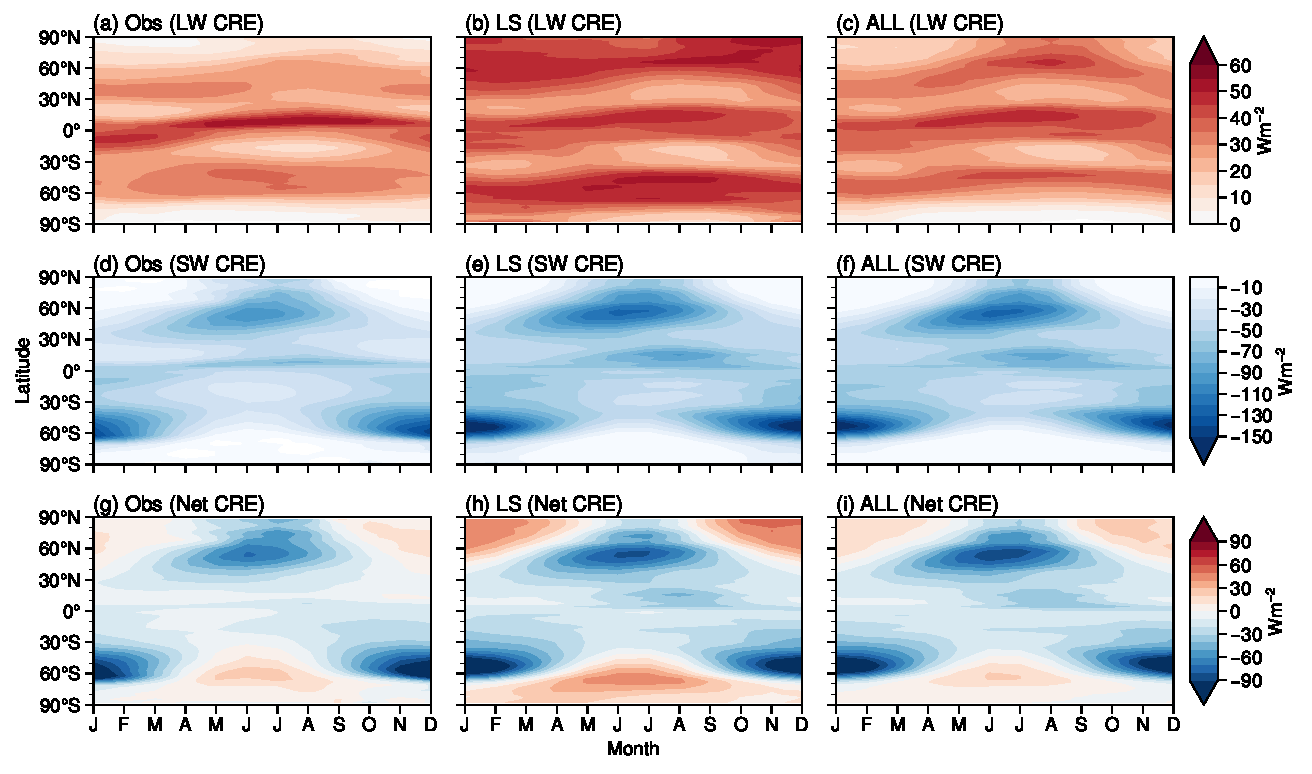
\includegraphics[width=1\linewidth]{{figs/evaluation_of_cld_scheme/isca_linear_amip_seasonal_cycle_map}.pdf}
	\caption{The zonal mean annual cycle of TOA LW (top), SW (middle) and net (bottom) CREs from observation (CERES-EBAF), LS and ALL simulations with the linear RH scheme in Isca.}
	\label{fig:cre_seasonal_cycle}
\end{figure}

The zonal mean seasonal cycles of CREs from CERES-EBAF and Isca simulations (LS and ALL) with the linear RH scheme are displayed in \figref{fig:cre_seasonal_cycle}. In the Arctic region, the observed LW CRE is weak during boreal winter and early spring, and has a maximum in summer (\figref{fig:cre_seasonal_cycle}a). The simulated LW CRE tends to be overestimated throughout the year in the LS run (\figref{fig:cre_seasonal_cycle}b), but the biases are alleviated by the freeze-dry adjustment (in the ALL run), particularly in winter (also see \figref{fig:cld_amt_freeze-dry}), leading to an overall improvement in the representation of the high-latitude seasonal cycle of the CRE. The existing problem for
the seasonal cycle of LW CRE is that the band in tropical region is too broad compared to the observations, which might relate to the too-broad high cloud pattern in tropical and subtropical regions (see \figref{fig:cld_fraction_profile}f). 

The seasonal cycle of SW CRE in the LS simulation is good, except that it is too strong during boreal summer near $60^\circ$N (\figsref{fig:cre_seasonal_cycle}d and \ref{fig:cre_seasonal_cycle}e). This effect is slightly mitigated in the ALL simulation (\ref{fig:cre_seasonal_cycle}f) because of the improvement of cloud amount. Similar to the LW CRE, the positive biases of net CRE in winter over polar regions are also alleviated due to the improvement of LW CRE in winter (\figsref{fig:cre_seasonal_cycle}h and \ref{fig:cre_seasonal_cycle}i). In summary, the seasonal cycles of LW, SW and net CREs in simulations with freeze-dry and inversion-based adjustments compare well to observations (left and right columns of \figref{fig:cre_seasonal_cycle}), indicating that the cloud scheme does reproduce a reasonably realistic seasonal cycle of CREs.


\subsection{Comparison with CMIP5 models}
\label{sec:cmp_cmip5}
\begin{figure}[ht]
	\centering
	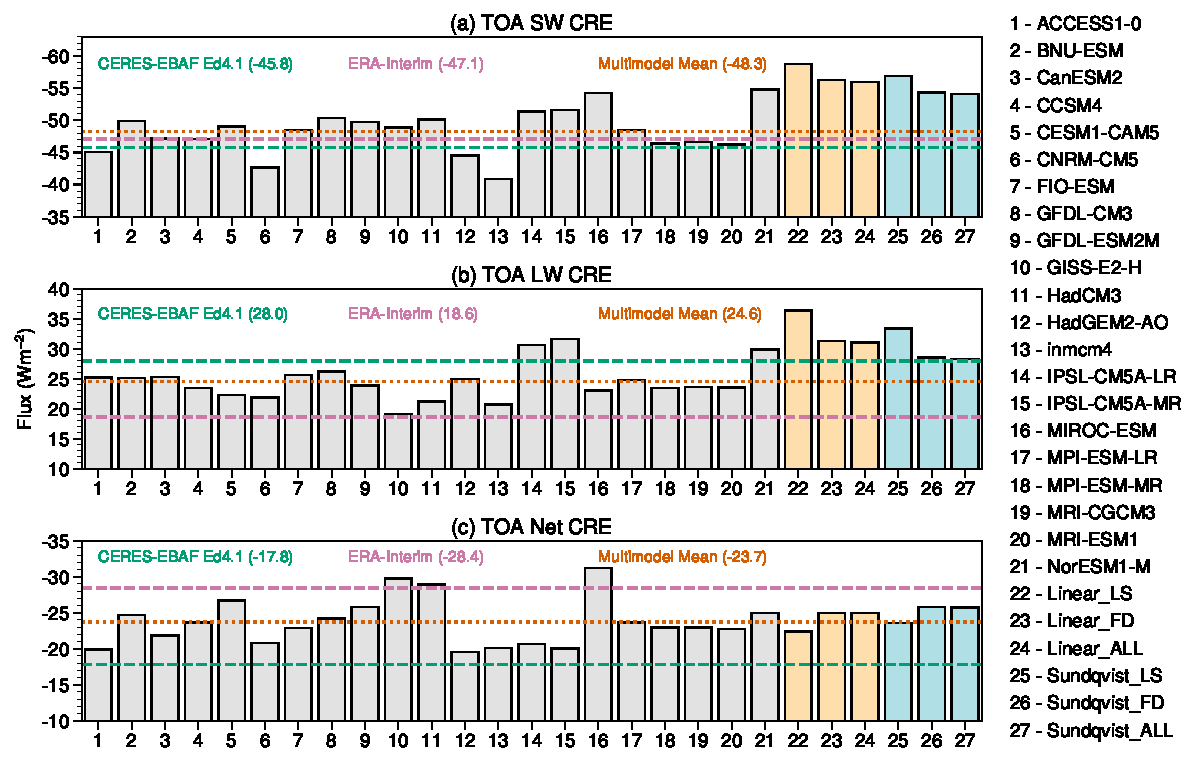
\includegraphics[width=1\linewidth]{{figs/evaluation_of_cld_scheme/global_mean_toa_CREs_4.1}.pdf}
	\caption{Globally averaged TOA (a) shortwave (SW), (b) longwave (LW) and (c) net cloud radiative effects (CREs, Wm$^{-2}$) from 21 CMIP5 models historical runs (1996-2005, gray bars) and Isca simulations with different setups (orange bars for linear scheme and cyan bars for Sundqvist scheme). The horizontal lines are annual and global mean CREs from CERES-EBAF (green dashed lines, covering from 2001 to 2018) and the multimodel ensemble mean results (orange dotted lines) of CMIP5 models, whose names are listed on right for reference.}
	\label{fig:global_mean_cres}
\end{figure}

\begin{figure}[ht]
	\centering
	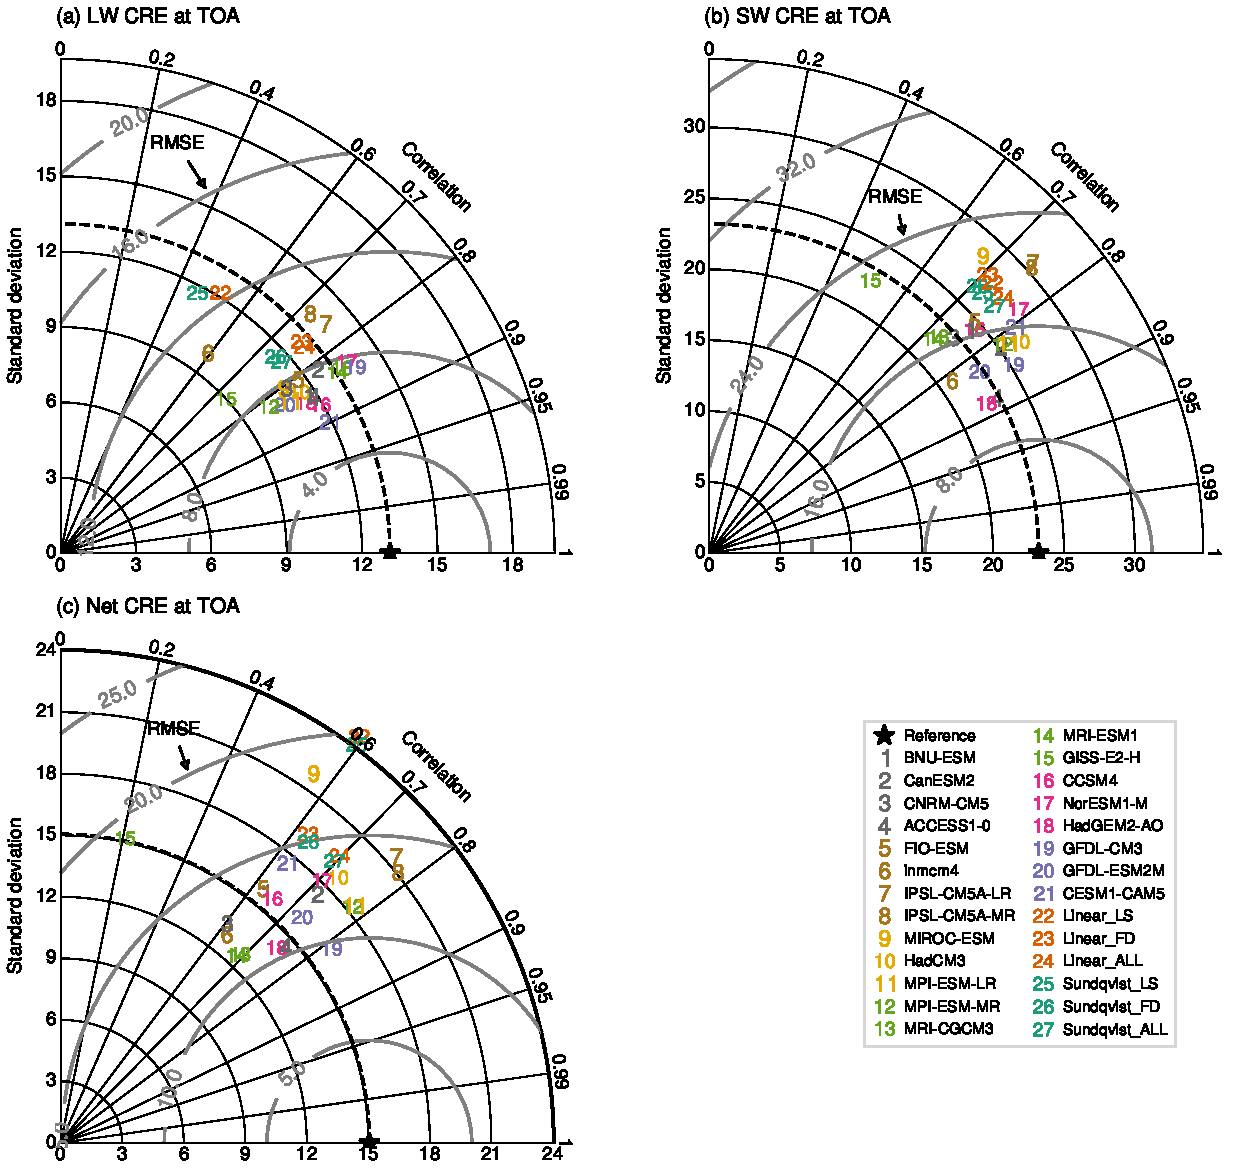
\includegraphics[width=1\linewidth]{{figs/evaluation_of_cld_scheme/cmp_cmip5_isca_CRE_taylor_obs_v4.1_sundqvist_linear}.pdf}
	\caption{Taylor diagrams showing standard deviation (Wm$^{-2}$), root mean square error (RMSE; Wm$^{-2}$) and spatial pattern correlation for the observed and simulated (a) LW, (b) SW and (c) net CREs at TOA in CMIP5 models and Isca simulations (LS, FD and ALL). The statistics of these variables are calculated based on annual mean data, where  the monthly data (1996-2005) from historical simulation is used for analysis of CMIP5 models. The observed field is as a reference and denoted by a black star. Contour of the standard deviation from observed field is shown by the black dashed line and contours of RMSE are displayed in gray with labels.}
	\label{fig:taylor_diagram}
\end{figure}

To evaluate the simulated CREs further, Isca simulations are compared with CMIP5 models. Figure \ref{fig:global_mean_cres} shows the global mean TOA SW, LW and net CREs from 21 CMIP5 models and Isca simulations with different cloud scheme setups. The observed SW CREs from CERES-EBAF and the multimodel mean of CMIP5 models are -45.8 Wm$^{-2}$ and -48.3 Wm$^{-2}$ respectively. While the multimodel mean SW CRE shows small difference from the observation, the spread among these CMIP5 models is large. Compared to the observation and CMIP5 models, the global mean SW CREs from the LS simulations with the linear RH and Sundqvist schemes are too strong, but they decrease in the FD and ALL simulations. With all components of our simple cloud scheme (ALL simulation), the global mean values are -56.0 and -54.1 Wm$^{-2}$ for linear RH and Sundqvist schemes respectively, which are fairly close to the observed and multimodel mean values. The changes of LW CRE from the LS to ALL simulations are similar to SW CRE, where it drops from 36.4 to 31.0 Wm$^{-2}$ for linear RH scheme and decreases from 33.3 to 28.3 Wm$^{-2}$ for Sundqvist scheme, making the results from simple cloud scheme closer to observations. These changes are probably due to the decrease of cloud fraction and cloud liquid water path discussed in sections \ref{sec:cld_amt} and \ref{sec:cwp}. The net CREs from all the Isca simulations are in a range that are comparable to the CMIP5 models, which are close to the multimodel mean but still over 7 Wm$^{-2}$ larger than CERES-EBAF.

We can also use a Taylor diagram \citep{Taylor2001} to compare Isca with other models, as this summarizes the standard deviation, pattern correlation and root mean square error (RMSE) in a single plot. Figure \ref{fig:taylor_diagram} shows the statistics of the observed and simulated LW, SW and net CREs from CMIP5 historical simulations (1996-2005) and Isca simulations. Compared to CMIP5 models, the LS runs from both the linear and Sundqvist schemes display large RMSEs and low spatial correlations for LW CRE field (\figref{fig:taylor_diagram}a), likely a consequence of too much clouds in polar regions. Similarly, the net CREs in the LS runs also show larger RMSEs and standard deviations than most CMIP5 models (\figref{fig:taylor_diagram}c). The FD and ALL simulations improve matters: going from the LS to FD simulations the RMSE decreases from 12.4 to 8.9 Wm$^{-2}$ and from 19.8 to 14.1 Wm$^{-2}$ for LW and net CREs respectively. For the SW CREs (\figref{fig:taylor_diagram}b), compared to the LS runs, the RMSEs in the ALL runs have decreased slightly in both linear and Sundqvist schemes.  By these metrics, the  simple cloud scheme  is evidently achieving a level of performance comparable to a number of CMIP5 models.


\section{Discussion and conclusions}

